\begin{itemize}
	
\item \textbf{Save User Route:}\\In this service contract, the code does obliged to all requested pertained in the conditions set out for this service contract. However the code does miss out on catering for the condition not stipulated which is the start saving a start point that is the same location as the end point.\\
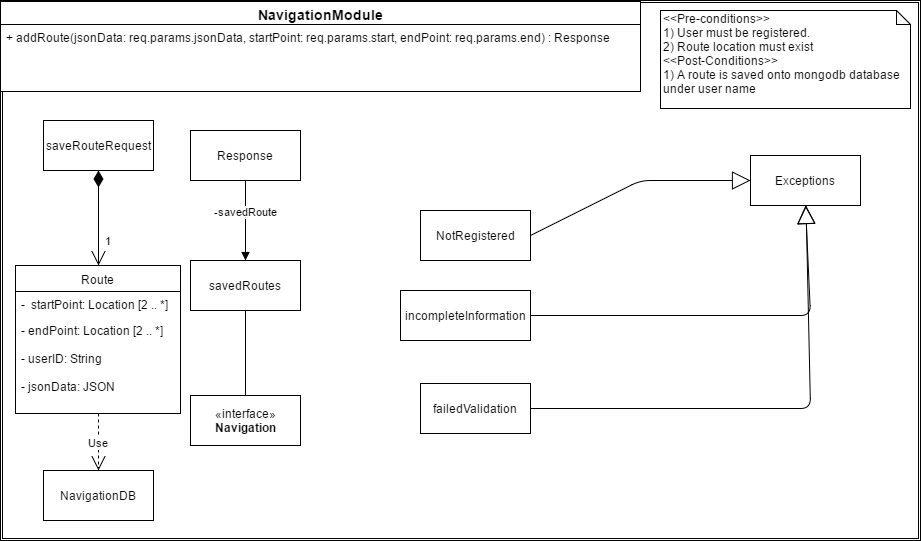
\includegraphics[scale=0.5]{SaveRoute.png}
\caption{Service Contract: Save User Preference}
	\textbf{Mark: 8/10}
	
\item \textbf{Save User Preference:}\\Service contract requires to save different preferences to a specific user when all Pre-Conditions are met. In this test, A discovery was made whereby the request overrides already existing preferences instead of appending new preferences or throw an exception if preference is used. This thus leads to it not fully fulfilling the service contract stipulated.\\
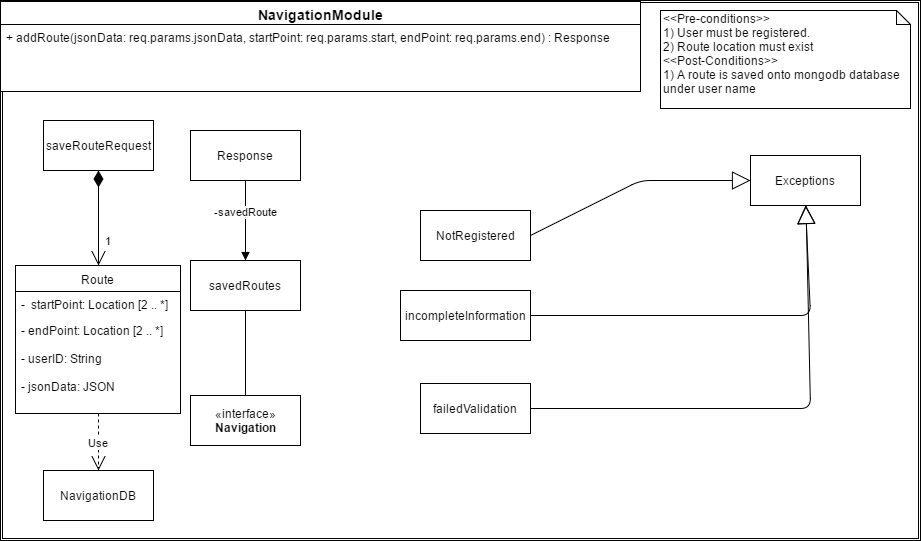
\includegraphics[scale=0.5]{SaveRoute.png}
\caption{Service Contract: Save User Preference}
	\textbf{Mark: 4/10}
\item \textbf{Cache Routes:}\\MongoDB as a choice of database management is favourable especially with regards scalability. However, the location data is not stored in a MongoDB database but rather in the same navigationLocal.js file as the entire program. This will cause a bottleneck when the amount of location data is increased.\\
	\textbf{Mark: 7/10}
	
\end{itemize}